\documentclass[12pt,a4paper]{article}
\usepackage[T1]{fontenc}
\usepackage[polish]{babel}
\usepackage{geometry}
\usepackage{fancyhdr}
\usepackage{graphicx}
\usepackage{booktabs}
\usepackage{float}

\geometry{margin=2.5cm}

\title{Projekt MPUM - Raport}
\author{Jakub Trela \and Karol Bielaszka}
\date{}

\pagestyle{fancy}
\fancyhf{}
\rhead{MPUM Projekt}
\lhead{Raport}
\cfoot{\thepage}

\begin{document}
\maketitle

\section*{Wstęp}
W naszym projekcie pracujemy nad datasetem {TODO wstaw ładny link do https://www.kaggle.com/datasets/irkaal/foodcom-recipes-and-reviews}. Zawiera on przepisy składające się z opisu dania, składników, instrukcji przygotowania, składników odrzywczych, calorii, liczby porcji dania itd. W naszych modelach będziemy rozważać jako argumnty jedynie instrukcje przygotowania dania ale przetestujemy też modele z dodakowym arguemnetm czyli liczbą porcji. Rozwarzając instrukcje przygotowania nie zwracamy uwagi na wartości liczb. Rozważamy jedynie słowa zawierające się w tekście. Będziemy przewidywać liczbę kalorii, tłuszczu, węglii i białek w rozważanych danych. Z racji, że samo zadanie jes dość skomplikowane, ponieważ w modelu 5g masła i 100g masła będą dokładnie tak samo interpretowane, nie spodziewamy się zbyt wysokich wyników. Jednak można założyć, że część informacji uda się wyciągąć, ponieważ na ogół przepisy zamieszone w internecie są przygotowywyane dla skończonej liczby osób (2-4). Zatem rozbierzność nie powinna być aż tak duża.

\subsection*{Porcje danych wybrane do trenowania modeli}
Do treningu danych używamy $120 000 - \epsi$ wierszy danych .

\section*{Analiza danych}
Nasz dataset składał się z wielu kolumn, my skupiliśmy się na przewidywaniu kalorii, węglowodanów, białka i tłuszczu na podstawie tekstowych instrukcji oraz liczby porcji (tylko niektóre modele). \\

\noindent Przykładowy wiersz z datasetu: \\

\begingroup
\small\ttfamily\noindent
Porcje: 4\quad Kalorie: 203.90 kcal\quad Tłuszcz: 7.30g\quad Węglowodany: 31.90g\quad Białko: 2.50g

\medskip
\noindent
Instrukcje: c("Pour cherry pie filling, cinnamon, cloves, and orange juice into a large pan.", "Add cherry liqueur and bring to a boil, stirring constantly.", "Scoop ice cream into sundae dishes.", "Top with hot cherries.")
\endgroup \\

\noindent Przy wczytywaniu danych pomijałem te które mają \texttt{NA} (brak danych) w conajmniej jednej z kolumn oraz te, które mają 0 we wszystkich kolumnach z wartościami liczbowymi (te wiersze wydawały się być wierszami z brakującymi danymi, ponieważ przepisy wyglądały normalnie).\\

\begin{table}[htbp]
    \centering
    \renewcommand{\arraystretch}{1.2}
    \begin{tabular}{|l|r|r|r|r|}
        \hline
        \textbf{Statystyka} & \textbf{Kalorie (kcal)} & \textbf{Tłuszcz (g)} & \textbf{Węglowodany (g)} & \textbf{Białko (g)} \\ \hline
        \textbf{Max} & 434 360.20 & 4 701.10 & 108 294.60 & 4 437.20 \\ \hline
        \textbf{98 perc.} & 1 209.63 & 77.80 & 118.00 & 63.80 \\ \hline
        \textbf{Średnia} & 371.82 & 18.76 & 34.99 & 15.96 \\ \hline
        \textbf{Mediana} & 291.20 & 12.70 & 25.90 & 8.90 \\ \hline
        \textbf{Odch. std.} & 878.20 & 31.94 & 193.74 & 24.61 \\ \hline
    \end{tabular}
    \caption{Statystyki opisowe wartości odżywczych (N = 337 685, śr. dł. instrukcji: 592.53 znaków)}
    \label{tab:statystyki_odzywcze_pion}
\end{table}

\noindent W datasecie występują wartości odstające, które mogą znacząco wpłynąć na wyniki analizy. W związku z tym zdecydowaliśmy się na obcięcie wartości do 98. percentyla. Poniżej znajdują się wykresy rozkładu dla każdej z analizowanych cech po obcięciu wartości odstających. Wykresy mają rozkłady skośne (im większe wartości, tym mniej danych), więc po prawej znajdują wykresy po zlogarytmowaniu, które przypominają rozkład normalny, co jest korzystne dla wielu modeli.

\begin{figure}[htbp]
    \centering
    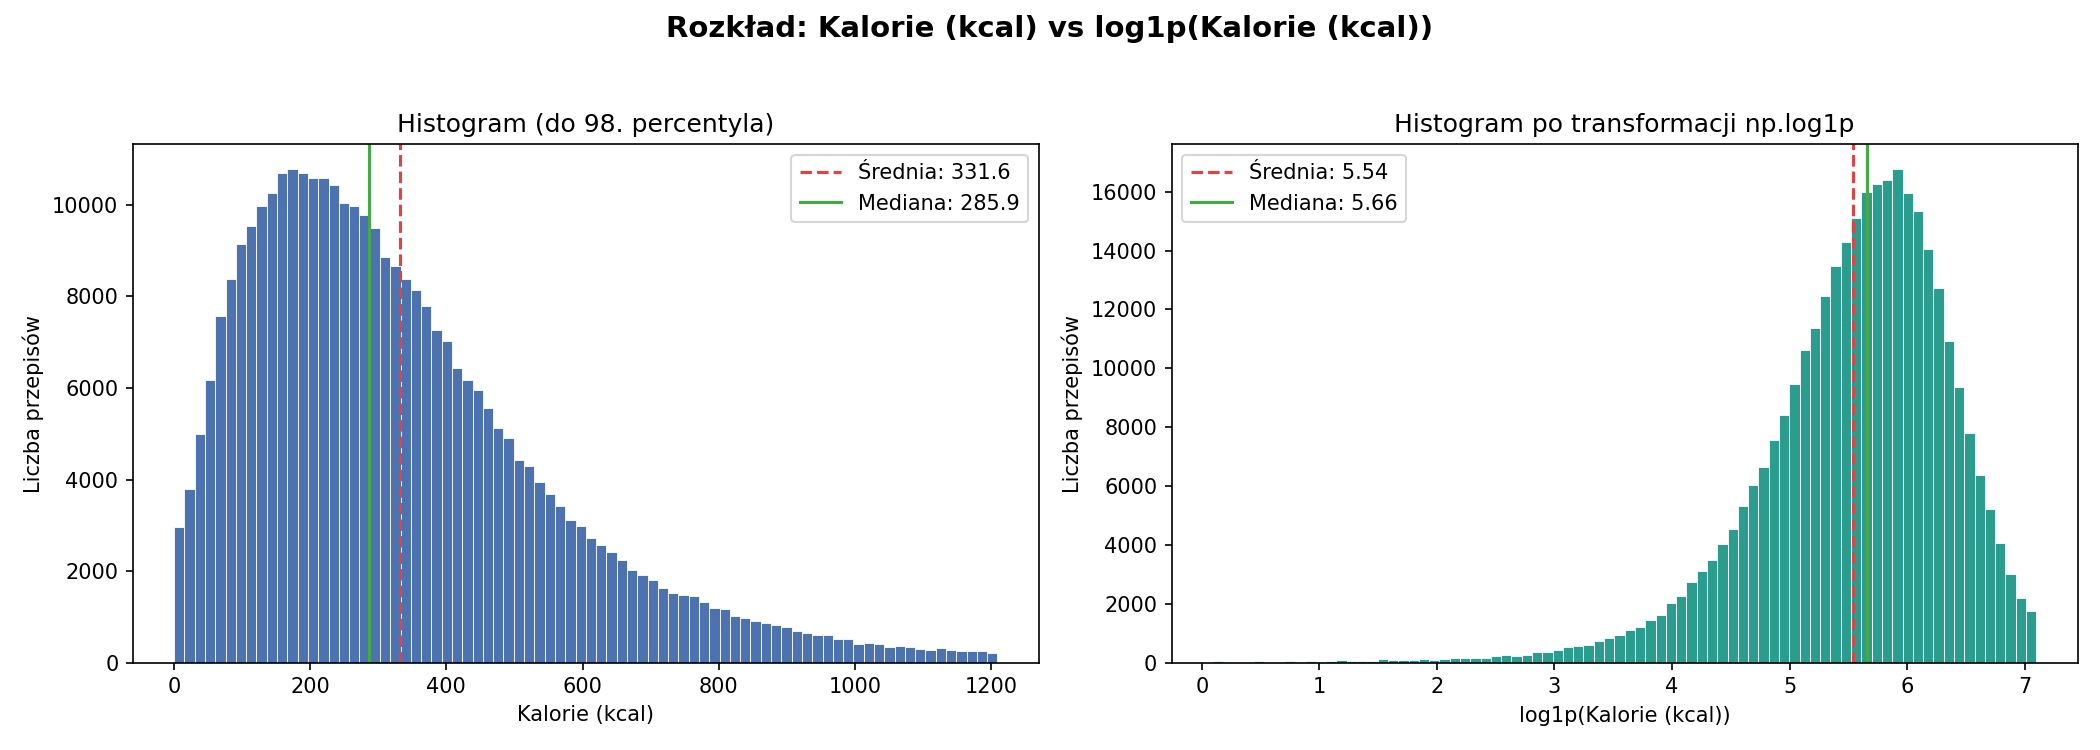
\includegraphics[width=0.8\textwidth]{img/calories_98.png}
    \caption{Rozkład kalorii w zbiorze danych.}
    \label{fig:calories_98}
\end{figure}

\begin{figure}[htbp]
    \centering
    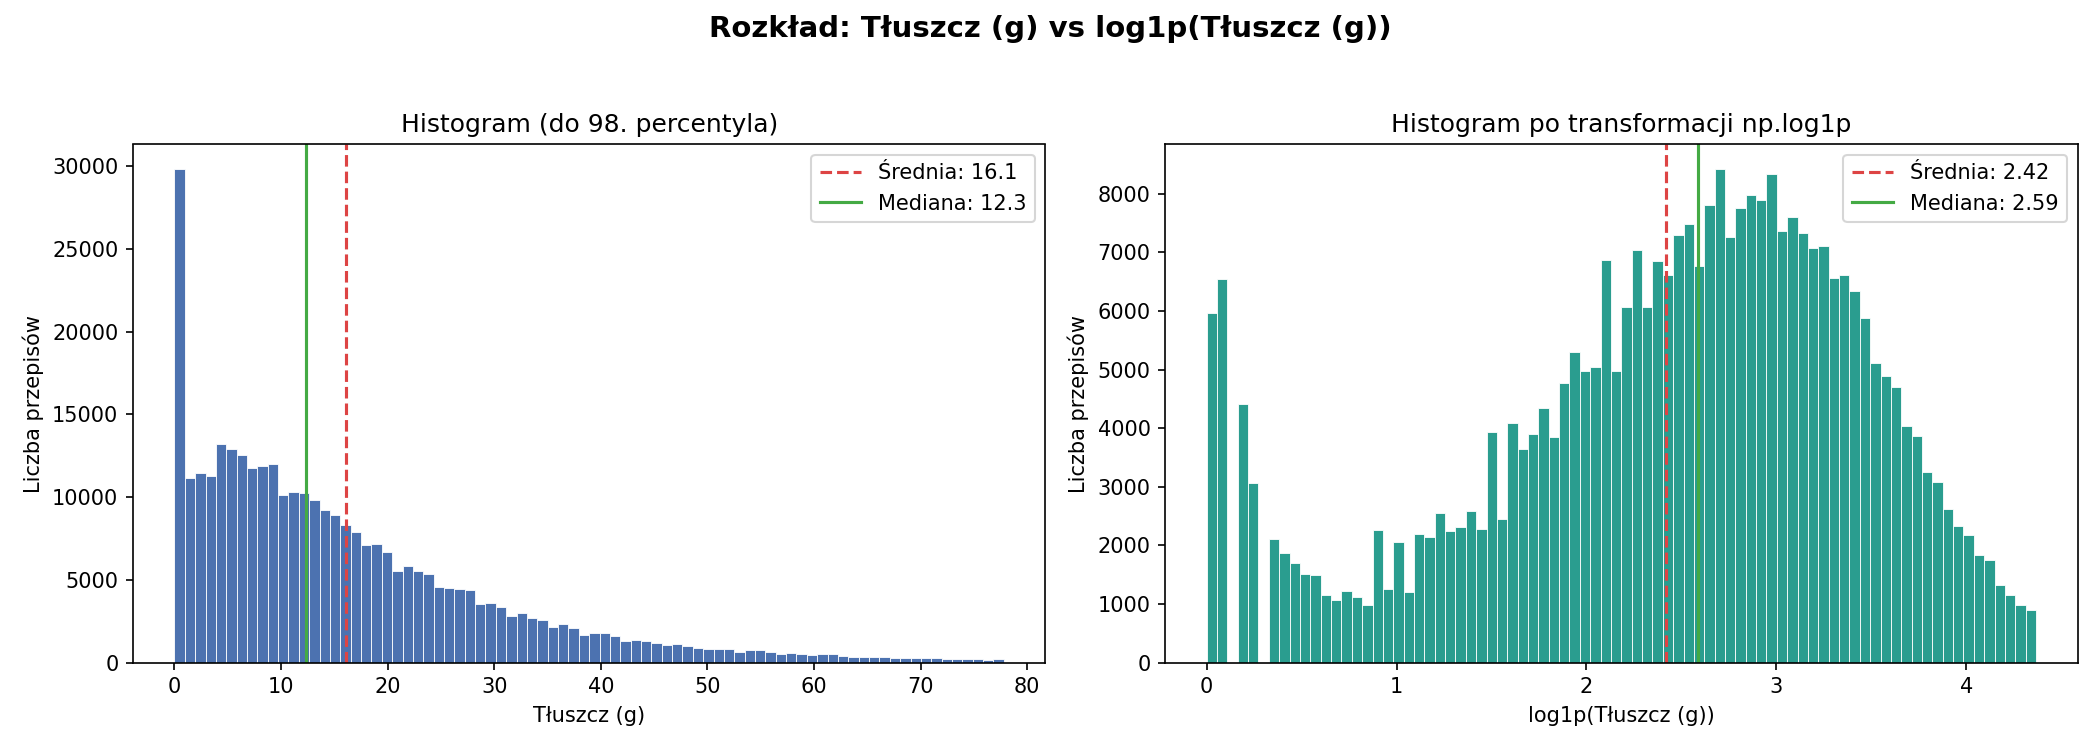
\includegraphics[width=0.8\textwidth]{img/fat_98.png}
    \caption{Rozkład tłuszczu w zbiorze danych.}
    \label{fig:fat_98}
\end{figure}

\begin{figure}[htbp]
    \centering
    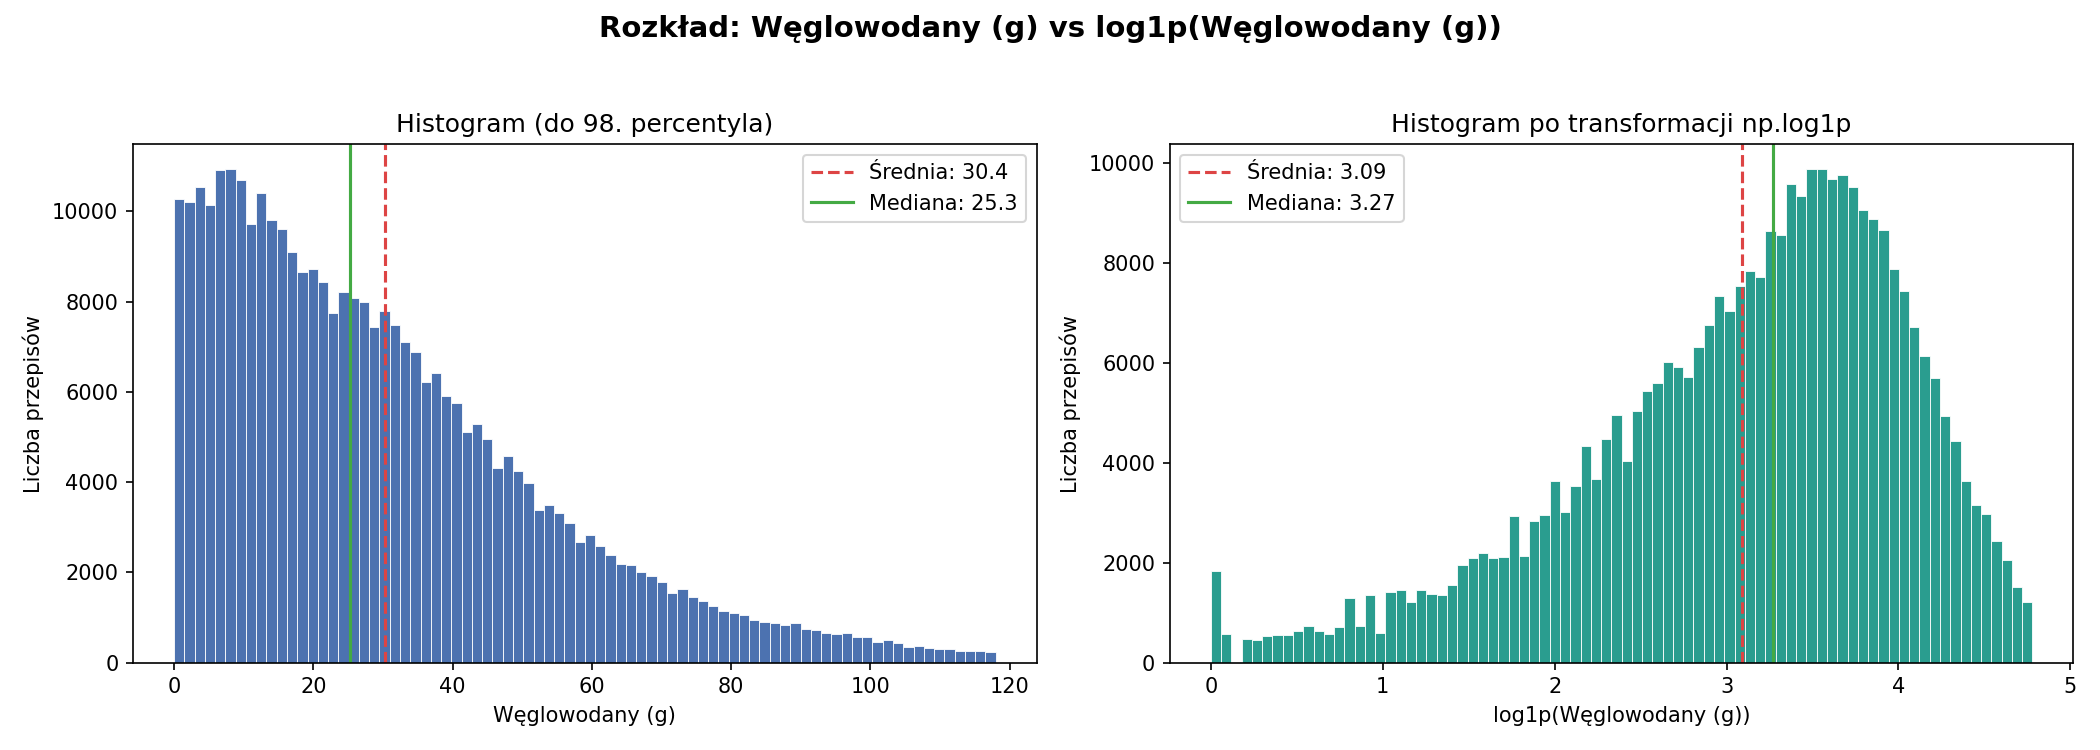
\includegraphics[width=0.8\textwidth]{img/carbohydrates_98.png}
    \caption{Rozkład węglowodanów w zbiorze danych.}
    \label{fig:carbohydrates_98}
\end{figure}

\begin{figure}[htbp]
    \centering
    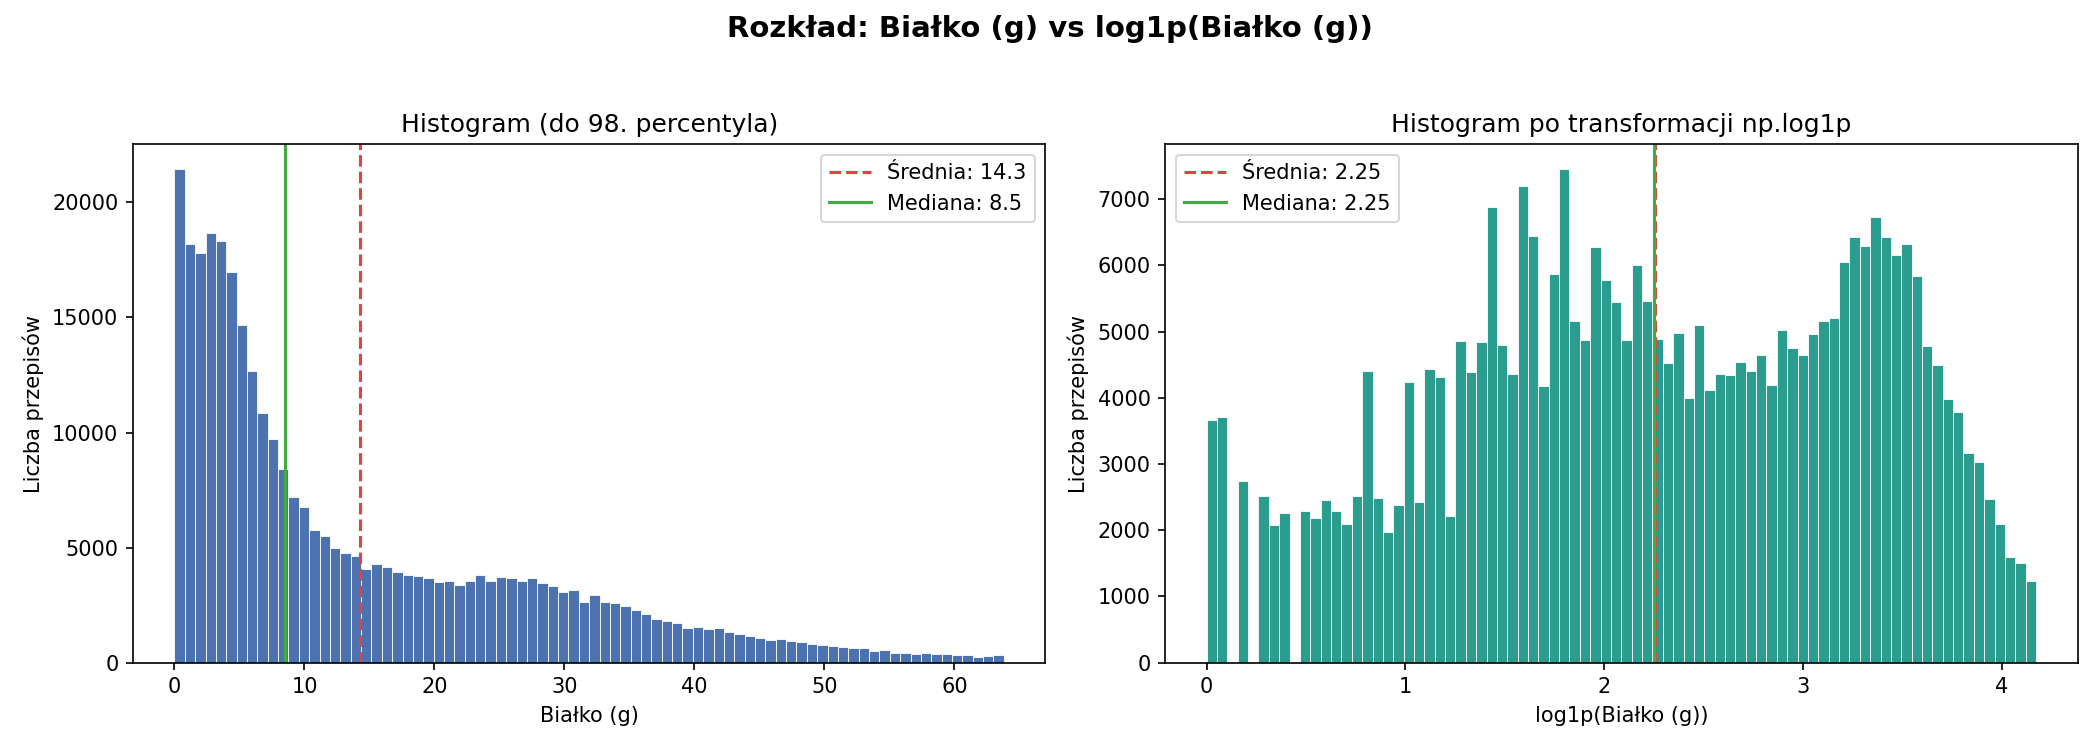
\includegraphics[width=0.8\textwidth]{img/protein_98.png}
    \caption{Rozkład białka w zbiorze danych.}
    \label{fig:protein_98}
\end{figure}

\section*{Ekstrakcja cech}

\subsection*{Tokenizacja}

Z tekstu usuwamy interpunkcję, liczby i znaki specjalne, a następnie dzielimy tekst na słowa.

\subsection*{Wektoryzacja}

Testujemy różne metody wektoryzacji:

\begin{itemize}
    \item Zwykłe zliczanie słów (Count Vectorizer) \\
        Polega na zliczaniu wystąpień poszczególnych słów w dokumencie.
    \item Term Frequency-Inverse Document Frequency (TF-IDF) \\
        Mierzy ważność słowa w dokumencie, uwzględniając jego częstość w całym korpusie. \\
        Term Frequency (TF) to liczba wystąpień słowa w dokumencie, a Inverse Document Frequency (IDF) to logarytmiczna odwrotność liczby przepisów zawierających to słowo. \\
        TF-IDF jest obliczane jako iloczyn TF i IDF.
    \item TF-IDF z cechami manualnymi \\
        Oprócz standardowego TF-IDF, dodajemy cechy takie jak liczba słów lub cechy dla różnych kategorii (np. fats and sweets, proteins, cooking methods heavy). Każda kategoria ma pewien zbiór słów kluczowych, których szukamy w tekście.
    \item Word2Vec \\
        Każde słowo jest reprezentowane jako wektor w przestrzeni wielowymiarowej, a dokument jest reprezentowany jako średnia wektorów słów w nim zawartych. Do wyliczenia wektorów trenujemy algorytm Word2Vec na naszym korpusie instrukcji.
\end{itemize}

    \noindent W Count i TF-IDF odrzucamy słowa, które występują w małej liczbie przepisów np. w mniej niż 3 przepisach oraz takie, które występują w bardzo dużej liczbie przepisów np. w więcej niż 90\% przepisów. Wybieramy też stałą liczbę cech (np. 5000) i bierzemy tylko te najczęściej występujące (Aby uniknąć zbyt dużej liczby cech, które mogą spowolnić działanie modelu). \\
    W tych 2 metodach używamy też bigramów (par słów występujących obok siebie). 

\subsection*{Porównanie metod wektoryzacji}

Metody te porównuje używając prostego modelu regresji liniowej z regularyzacją L2 (Ridge) i porównując średni błąd bezwzględny (MAE), pierwiastek średniego błędu kwadratowego (RMSE) i współczynnik determinacji ($R^2$). \\
($R^2$ mówi nam, jak model jest lepszy niż prosty model, który zawsze przewiduje średnią wartość. $R^2$ = 0 oznacza, że model jest tak dobry jak ten prosty model, a $R^2$ = 1 oznacza idealne dopasowanie do danych).\\

\noindent Ponieważ wykresy rozkładu cech są skośne to modele przewidują logarytm wartości, a następnie bierzemy wykładnik z przewidywań, aby otrzymać przewidywane wartości. \\

\begin{table}[htbp]
    \centering
    \caption{Wyniki ewaluacji modeli na zbiorze Walidacyjnym}
    \label{tab:wyniki_wektoryzacji_val}
    \renewcommand{\arraystretch}{1.2}
    \begin{tabular}{|l|l|r|r|r|}
        \hline
        \textbf{Metoda} & \textbf{Zmienna docelowa} & \textbf{MAE} & \textbf{RMSE} & \textbf{$R^2$} \\ \hline
        
        \textbf{Count} & Calories & 144.968 & 220.498 & 0.0309 \\ 
        & Fat & 9.711 & 19.886 & -0.6010 \\ 
        & Carbohydrates & 16.910 & 35.965 & -1.0373 \\ 
        & Protein & 8.221 & 15.138 & -0.0421 \\ \hline
        
        \textbf{TF-IDF} & Calories & 135.859 & 193.744 & 0.2518 \\ 
        & Fat & 8.801 & 13.839 & 0.2246 \\ 
        & Carbohydrates & 15.344 & 22.762 & 0.1840 \\ 
        & Protein & 7.053 & 11.411 & 0.4079 \\ \hline
        
        \textbf{TF-IDF + Manual} & Calories & 134.645 & 191.838 & 0.2664 \\ 
        & Fat & 8.676 & 13.678 & 0.2426 \\ 
        & Carbohydrates & 15.093 & 22.465 & 0.2051 \\ 
        & Protein & 7.018 & 11.381 & 0.4110 \\ \hline
        
        \textbf{Word2Vec} & Calories & 151.638 & 214.352 & 0.0842 \\ 
        & Fat & 9.926 & 15.258 & 0.0574 \\ 
        & Carbohydrates & 16.995 & 24.716 & 0.0378 \\ 
        & Protein & 8.100 & 12.852 & 0.2489 \\ \hline
    \end{tabular}
\end{table}

\noindent Proste zliczanie radzi sobie bardzo słabo, nawet gorzej od modelu, który zawsze przewiduje średnią wartość. TF-IDF daje znaczną poprawę, a dodanie cech manualnych daje jeszcze niewielką poprawę. Word2Vec radzi sobie gorzej niż TF-IDF, co może być spowodowane tym, że średnia wektorów słów może nie być najlepszym sposobem reprezentacji całego przepisu. \\ 

\noindent Warto zauważyć że przewidywanie ilości białka jest łatwiejsze niż przewidywanie kalorii oraz pozostałych makroskładników.

\section*{Regresja z regularyzacją}

Przetestowaliśmy analityczna regresję liniową z regularyzacją L2 (Ridge) oraz regrsję z siecią elastyczną (ElasticNet) z gradient descent. Poniżej znajdują się wyniki współczynnika determinacji ($R^2$) dla różnych wartości parametów regularyzacji. (Im więcej tym lepiej) \\

\begin{figure}[H]
    \centering
    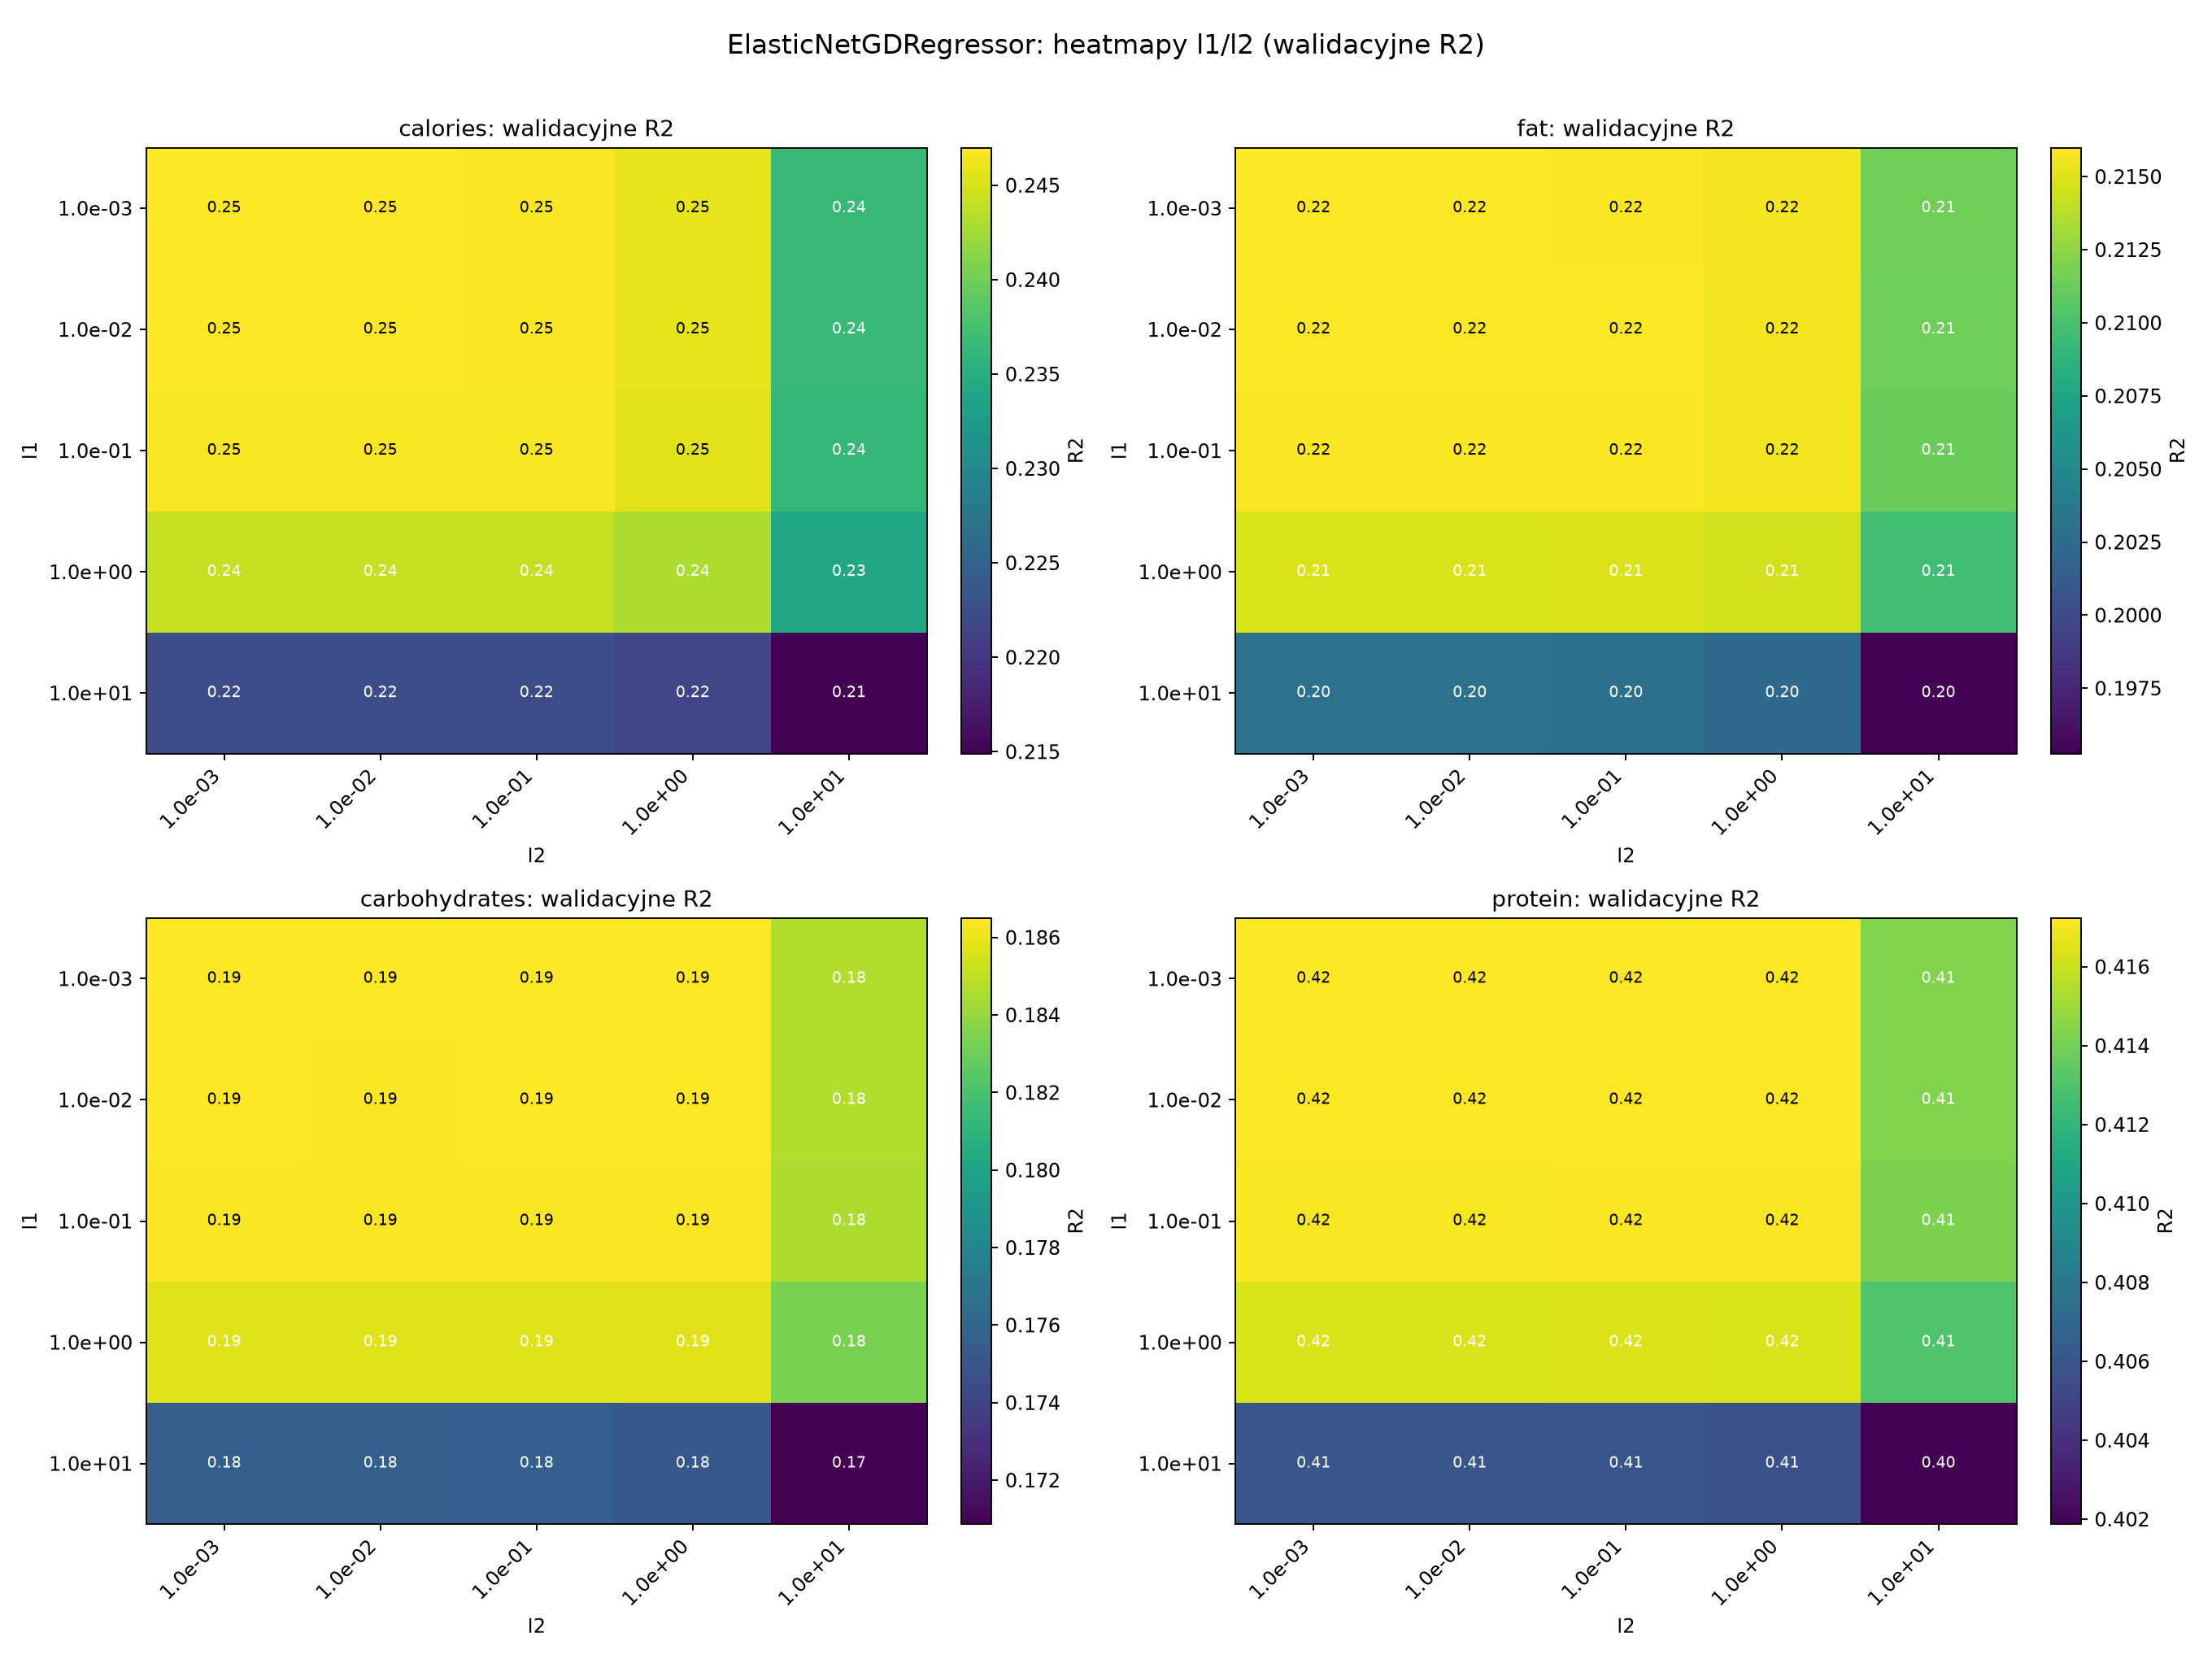
\includegraphics[width=\textwidth]{img/regularization_heatmaps.png}
    \caption{Współczynnik ($R^2$) dla regresji Elastic Net w zależności od parametrów regularyzacji l1 i l2.}
    \label{fig:elasticnet_regularization}
\end{figure}

\begin{figure}[H]
    \centering
    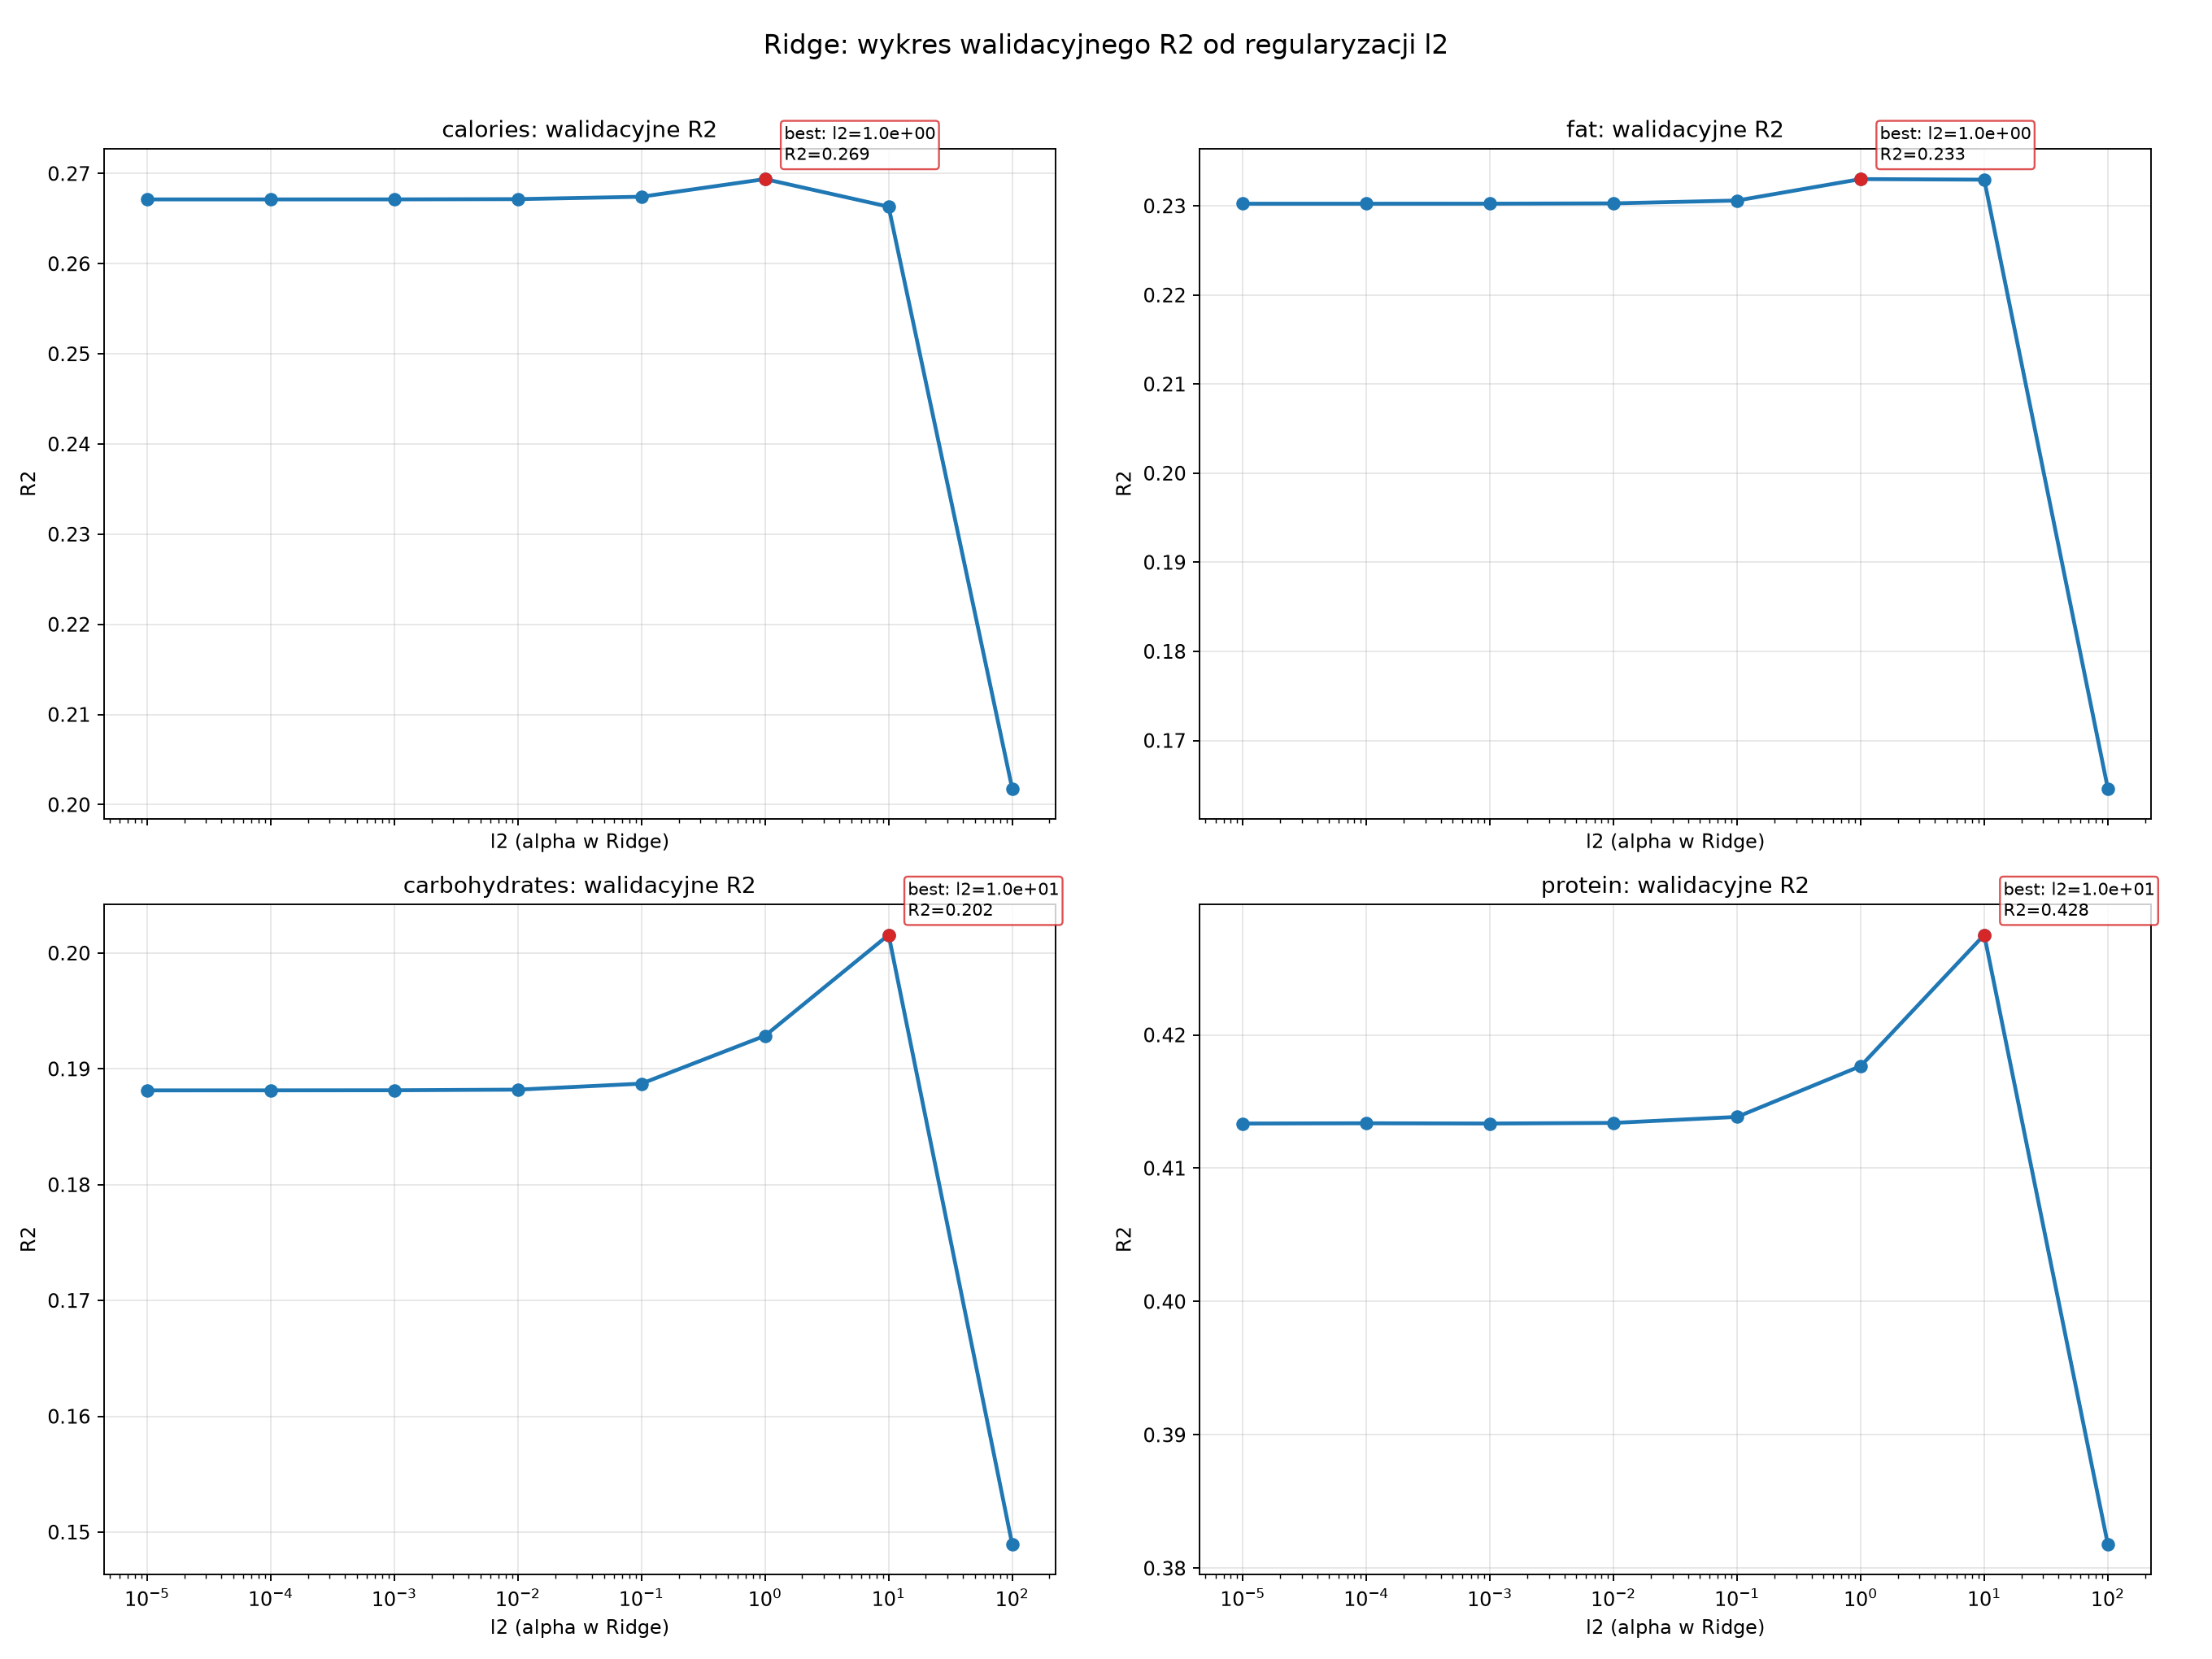
\includegraphics[width=\textwidth]{img/regularization_plot.png}
    \caption{Współczynnik ($R^2$) dla regresji Ridge w zależności od parametru regularyzacji l2.}
    \label{fig:ridge_regularization}
\end{figure}

\noindent W regresji Elastic Net najlepiej sprawdzają się małe wartości regularyzacji, a w regresji Ridge najlepiej sprawdzają się wartości 1 lub 10, w zalezności od zmiennej docelowej. \\

\noindent Wyniki regresji Ridge są nieco lepsze niż Elastic Net, prawdopodobnie dlatego, że rozwiązanie analityczne jest dokłądniejsze niż gradient descent, który może nie znaleźć najlepszego rozwiązania. \\

\end{document}